\subsection{Scenarios Used for the Simulations}
All simulations considered in this second part were extended to 2130, where the forcing was kept constant at the 2100 levels. This extension provides further insight in the long-term effects of deploying SAI. Especially in the rapid cooling SAI scenario the extension provides time for the climate system to adjust to the `shock' it experienced from SAI. 

Shown in Figure \ref{fig:Tgrad_ext} are the temperature targets from Equation \ref{eq:Tpsi} for the SSP5-8.5, gradual SAI and rapid cooling SAI simulations. After about 10 years of SAI the $T_0$ target is reached and maintained, like in the gradual SAI simulation. However, in contrast to the gradual SAI simulation, the rapid cooling SAI simulation is not able to return to and then maintain 2020 levels for $T_1$ and $T_2$. In the rapid cooling SAI simulation both targets are overshot, though their levels are stabilised after 2100. 

\begin{figure}[h]
	\centering
	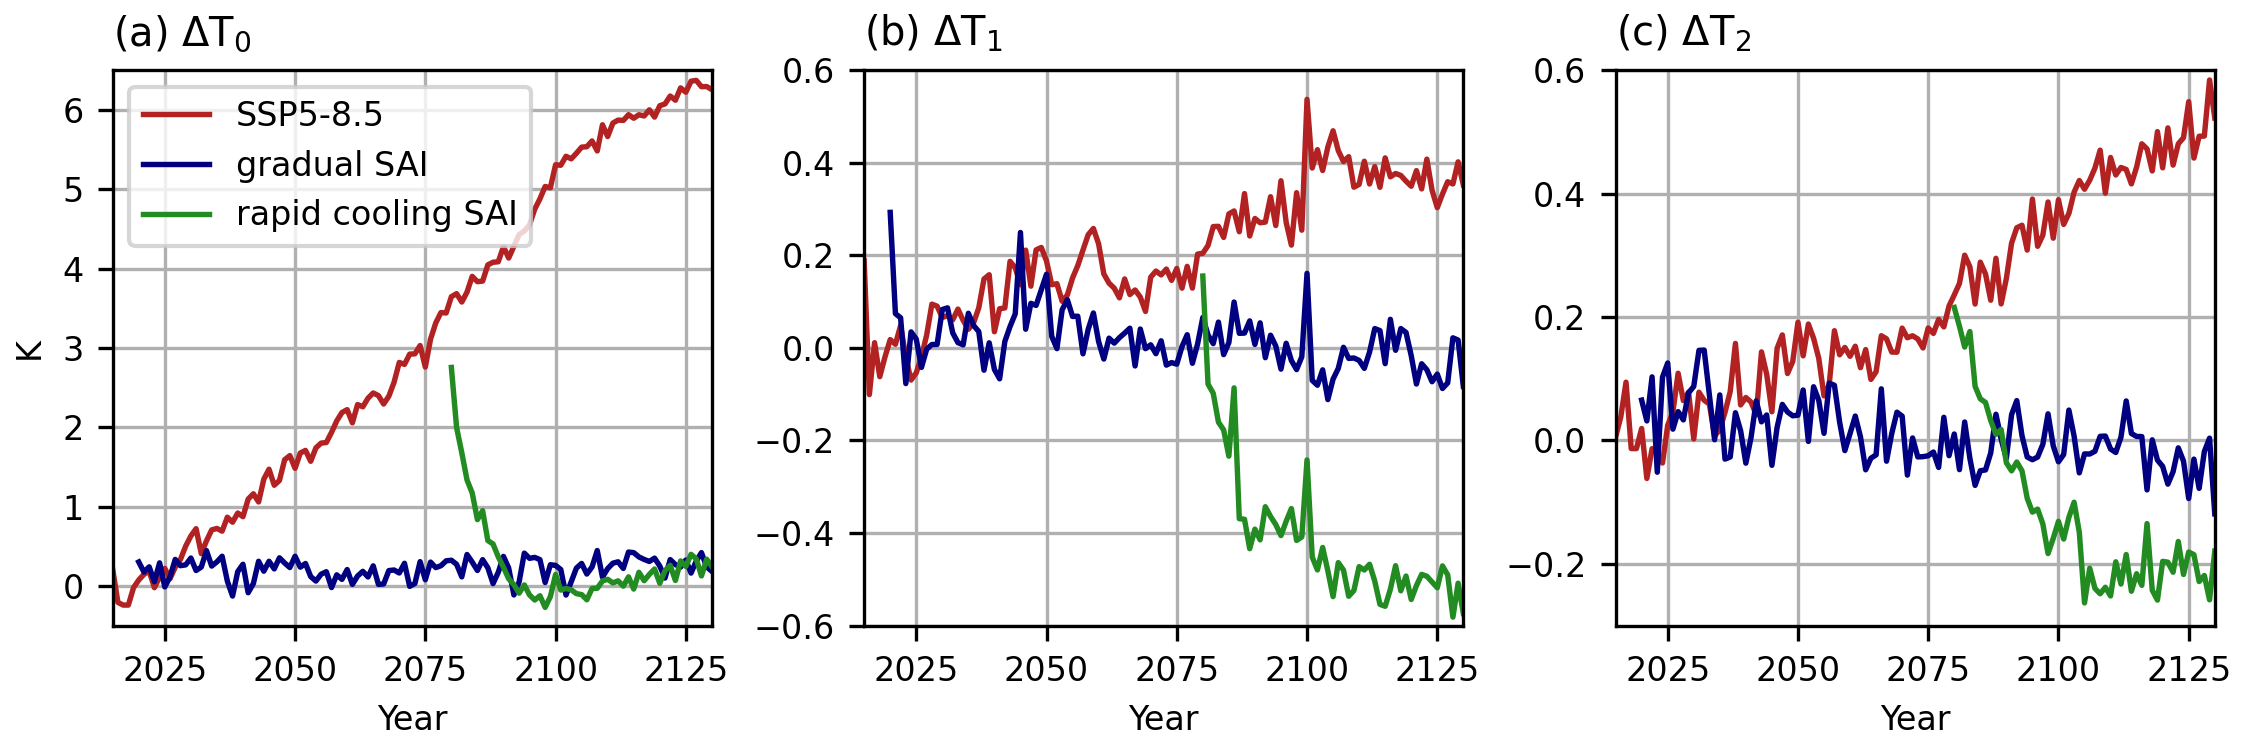
\includegraphics[width=\linewidth]{images/Tgrad_ext.png}
	\caption{Deviatons from temperature targets $T_0$, $T_1$, $T_2$ as compared to 2016-2025 mean, for Control, SAI 2020 and SAI 2080 scenarios in CAM.}
	\label{fig:Tgrad_ext}
\end{figure}


\subsection{Definition of Scenarios and Time Periods for Part II}
Throughout this second part, four time periods are selected to visualise and interpret the results from the simulations. As in part I, for each period the 20-year mean is taken, unless specified otherwise. These periods are defined as follows:

\begin{itemize}
    \item \textbf{Reference} The period 2016-2035 of the SSP5-8.5 simulation.
    \item \textbf{Control} The period 2111-2130 of the SSP5-8.5 simulation.
    \item \textbf{SAI 2020} The period 2111-2130 of the gradual SAI simulation.
    \item \textbf{SAI 2080} The period 2111-2130 of the rapid cooling SAI simulation.
\end{itemize} % tabel van maken


\subsection{Thermal Wind}
The thermal wind is the vertical shear due to horizontal temperature variations. We can calculate the wind as the result of such temperature variations in the zonal and meridional direction through the thermal wind balance. With the vertical layers of the model converted to pressure coordinates, this equation takes the form 

\begin{equation}
    \frac{\partial v_g}{\partial p} = - \frac{R}{pf_0} \frac{\partial T}{\partial x};\ 
    \frac{\partial u_g}{\partial p} = \frac{R}{pf_0} \frac{\partial T}{\partial y},
\end{equation}

where $v_g$,$u_g$ is the geostrophic wind in meridional and zonal directions respectively, $R = 286.9$ J kg$^{1}$ K$^{1}$ is the specific gas constant for dry air, $p$ is pressure, $f_0 = 2\Omega \sin \varphi$ is the coriolis parameter at the chosen reference latitude $\varphi$, $\frac{\partial T}{\partial x,y}$ is the layer-mean temperature gradient in zonal and meridional direction respectively. Rewriting and integrating gives us

\begin{equation}
    \begin{split}
        \int\displaylimits_{p_0}^{p_1} \partial v_g &= \int\displaylimits_{p_0}^{p_1} - \frac{R}{f_0} \frac{\partial T}{\partial x} \partial \ln p; \\
        \int\displaylimits_{p_0}^{p_1} \partial u_g &= \int\displaylimits_{p_0}^{p_1} \frac{R}{f_0} \frac{\partial T}{\partial y} \partial \ln p,
    \end{split}
\end{equation}

where $p_{0,1}$ are the lower and upper boundaries of the model layer, respectively, so that $p_1 < p_0$. Because $T$ is the layer-mean temperature and $R$ and $f_0$ are constants, we can evaluate this integral to find the thermal wind in the layer between $p_0$ and $p_1$

\begin{equation}
    \begin{split}
        v_T = v_g(p_1) - v_g(p_0) &= \frac{R}{f_0} \frac{\partial T}{\partial x} \ln\left(\frac{p_0}{p_1}\right);\\
        u_T = u_g(p_1) - u_g(p_0) &= - \frac{R}{f_0} \frac{\partial T}{\partial y} \ln\left(\frac{p_0}{p_1}\right).
    \end{split}
\end{equation}

To increase stability in our calculations, we assume that the thermal wind below 850 hPa is equal to the model wind, because the thermal wind calculation in the layers below that will most likely not produce stable results. To then find the integrated thermal wind at a given pressure coordinate above 850 hPa, we take the cumulative sum of the thermal wind from 850 hPa up to the given pressure plus the meridional or zonal wind of the layer below 850 hPa ($v(p_{<850}),u(p_{<850})$). This gives us for the integrated thermal wind at pressure coordinate $p_i$ 

\begin{equation}
    \begin{split}
        v_{T}(p_i) &= v(p_{<850}) + \frac{R}{f_0} \sum_{i=0}^{i} \frac{\partial T_i}{\partial x} \ln \left(\frac{p_i}{p_{i+1}}\right),\\
        u_{T}(p_i) &= u(p_{<850}) + \frac{R}{f_0} \sum_{i=0}^{i} - \frac{\partial T_i}{\partial y} \ln \left(\frac{p_i}{p_{i+1}}\right).
    \end{split}
\end{equation}


\subsection{Kinetic Energy and Eddy Kinetic Energy}
The CAM model woks with wind in the form of $u = \overline{u} + u^{\ast}$, $v = \overline{v} + v^{\ast}$, with $u,v$ the total wind, $\overline{u},\overline{v}$ the monthly-mean wind and $u^\ast,v^\ast$ the deviation from the mean wind. The model output contains monthly averages $\overline{u},\overline{v}$ and $\overline{u^2},\overline{v^2}$. % check in CESM documentation

The kinetic energy $KE$ per unit mass can thus be found from the model results directly through

\begin{equation}\label{eq:KE}
    KE = \frac{1}{2} \left( \overline{u^2} + \overline{v^2} \right).
\end{equation}

The eddy kinetic energy $EKE$ per unit mass can be found through 

\begin{equation}\label{eq:EKE}
    EKE = \frac{1}{2} \left( \overline{u^{\ast 2}} + \overline{v^{\ast 2}} \right),
\end{equation}

\noindent with $\overline{u^{\ast 2}}, \overline{v^{\ast 2}}$ found through
\begin{equation}
    \begin{split}
        \overline{u^2} &= \overline{\left( \overline{u} + u^\ast \right) \left( \overline{u} + u^\ast \right)},\\
        &= \overline{\overline{u}^2 + 2 \overline{u}u^\ast + u^{\ast 2}},\\
        &= \overline{u}^2 + \overline{u^{\ast 2}} \Rightarrow \overline{u^{\ast 2}} = \overline{u^2} - \overline{u}^2, 
    \end{split}
\end{equation}

which can be found with the model output. 

To find the kinetic and eddy kinetic energy per unit volume, we multiply the results from Eq. \ref{eq:KE} and \ref{eq:EKE} with the local density. Assuming an ideal gas, we approximate the density through
\begin{equation}
    \rho = \frac{p}{RT},
\end{equation}
\noindent with $p$ pressure, $T$ temperature and $R$ again the specific gas constant for dry air. 


\subsection{Jet Intensity Maps}
To visualise the extent and intensity of an atmospheric jet, we introduce the jet intensity map. The map is made by counting the number of times the zonal wind or eddy kinetic energy surpasses a set threshold. Each timestep and coordinate is evaluated individually, after which the set is summed over time and the vertical dimension. This result is then normalised to the total the number of timesteps multiplied by the number of vertical model levels included in the analysis. This results in a fraction that represents the occurence and vertical extent of the atmospheric jet. The threshold is chosen to be about 80\% of the maximum of the zonal mean.

To visualise the Polar night jet (PNJ), in the upper stratosphere, and the subtropical jet (STJ), in the lower stratosphere, this method is applied to the zonal wind fields. For the eddy-driven jet (EDJ), also in the lower stratosphere, this method is applied to the eddy kinetic energy fields. For all jets the threshold and vertical selection are noted in the figure description. 

\subsection{Sudden Stratospheric Warmings in Monthly Mean Model Data}
Typical metrics for SSWs rely on daily model data to identify an event. Metrics typically use the reversal of zonal-mean zonal wind at 10 hPa and 60°N/S, form westerly to easterly, the reversal of the meridional temperature gradient at 10 hPa above 60°N/S, changes in the geopotential height field or topology of the polar vortex, or a combination and/or variation of these. Additionally, metrics typically include temporal constraints, excluding events that occur within a certain number of days of another event, or events after which the atmosphere does not return to its winter state (final warming) before the end of the season \parencite{butler2015}. 

Because we consider monthly mean data these metrics are inapplicable. We therefore use a modified approach. we consider the zonal-mean zonal wind at 10 hPa and 60°S and the area-weighted average temperature at 10 hPa above 60°S. We consider the atmosphere to be in an SSW-like state when the zonal wind decreases or the temperature increases significantly in the winter months.